88. Для построения графика функции $f(x)=|x^2-6x+5|$ сначала построим параболу $y=x^2-6x+5=(x-1)(x-5).$ После этого отразим её отрицательную часть при $x\in(1;5)$ наверх относительно оси абсцисс. Её вершина $(3;-4)$ отразится в точку $(3;4).$ График функции $g(x)=k(x-7)+4$ при любом значении $k$ проходит через точку $(7;4).$  С графиком функции $f(x)$ он может иметь три общие точки только в двух случаях: если параллелен оси абсцисс, тогда $k=0,$ или если проходит через точку $(1;0),$ в этом случае $0=k\cdot(-6)+4,\ k=\cfrac{2}{3}.$
$$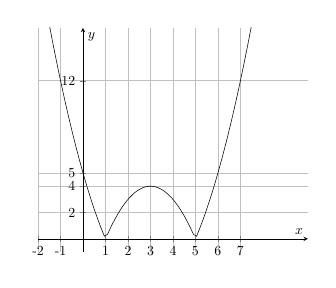
\begin{tikzpicture}[scale=0.5]
\begin{axis}[
    axis lines = middle,
    grid=major,
    legend pos={south west},
    xlabel = {$x$},
    %xlabel style={below right},
    ylabel = {$y$},
    ymin=-1,
    ymax=16,
    xmin=-2,
    xmax=10,
    xtick={-2,-1,1,2,3,4,5,6,7},
    xticklabels={-2,-1,1,2,3,4,5,6,7},
    ytick={2,4,5,12},
    yticklabels={2,4,5,12},
                  ]
	\addplot[domain=-4:10, samples=100, color=black] {abs(x*x-6*x+5)};
        %\addplot[domain=2.01:6, samples=100, color=black] {2/(2-x)};
   % \addplot[domain=-3:3, samples=100, color=black] {-x};
     %\addlegendentry{$\text{Рис. 1}$};
\end{axis}
\end{tikzpicture}$$
